\input{configuration}

\title{Lecture 26 --- Finding Bottleneck Devices}

\author{Jeff Zarnett\\ \small \texttt{jzarnett@uwaterloo.ca}}
\institute{Department of Electrical and Computer Engineering \\
  University of Waterloo}
\date{\today}


\begin{document}

\begin{frame}
  \titlepage

\end{frame}

\begin{frame}
\frametitle{Bug Reports}

\begin{center}
  
\includegraphics[width=0.5\textwidth]{images/onestar.jpg}
\end{center}

Poor mobile app performance is a major complaint in app store reviews.

\end{frame}

\begin{frame}
\frametitle{Real Bug Report}

\begin{center}
  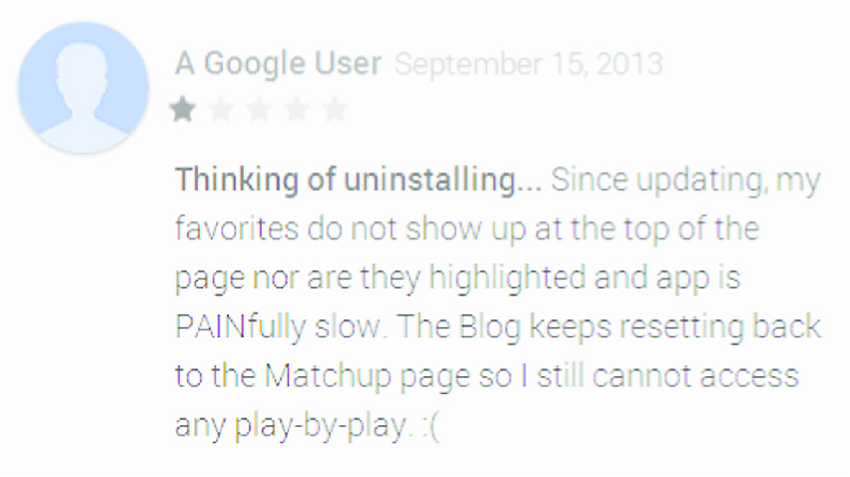
\includegraphics[width=0.5\textwidth]{images/slow-app.png}
\end{center}

We might have a \textit{vague} idea what's wrong, but how do we fix it?

\end{frame}


\begin{frame}
\frametitle{Who Can It Be Now?}

\begin{center}
	\includegraphics[width=0.6\textwidth]{images/n-body-go-brrrrr.png}
\end{center}

We usually assume that CPU is the problem... but is that true?

Future topics will mostly follow CPU profiling, but it's not the only thing.

\end{frame}




\begin{frame}
\frametitle{Elementary, My Dear Watson!}



\begin{quote}
\textit{It is a capital mistake to theorize before one has data. Insensibly one begins to twist facts to suit theories, instead of theories to suit facts.}
\end{quote}
\hfill --- Sherlock Holmes\\
\hfill (\textit{A Scandal in Bohemia}; Sir Arthur Conan Doyle)


\begin{center}
	\includegraphics[width=0.3\textwidth]{images/jeremybrett.jpg}
\end{center}

\end{frame}



\begin{frame}
\frametitle{Collect Evidence}



Who's to blame?
\begin{enumerate}
	\item CPU
	\item Memory
	\item Disk
	\item Network
	\item Locks
\end{enumerate}

These are, obviously, \\
categories rather than specific causes.

\end{frame}

\begin{frame}
\frametitle{How to Fix It?}

Fixing it might involve using techniques from this course...\\
\quad But it might be really difficult.

Is the user's hardware just too old?

\begin{center}
  
\includegraphics[width=0.6\textwidth]{images/hulk.jpg}
\end{center}

\end{frame}

\begin{frame}
\frametitle{It's a bug?}

The ``slow'' workflow might actually be a bug...

Are you doing a slow or async task in the UI thread?

Oops! Just fix the bug.

\end{frame}



\begin{frame}
\frametitle{Blame the CPU}



CPU is probably the easiest of these to diagnose.

\begin{center}
  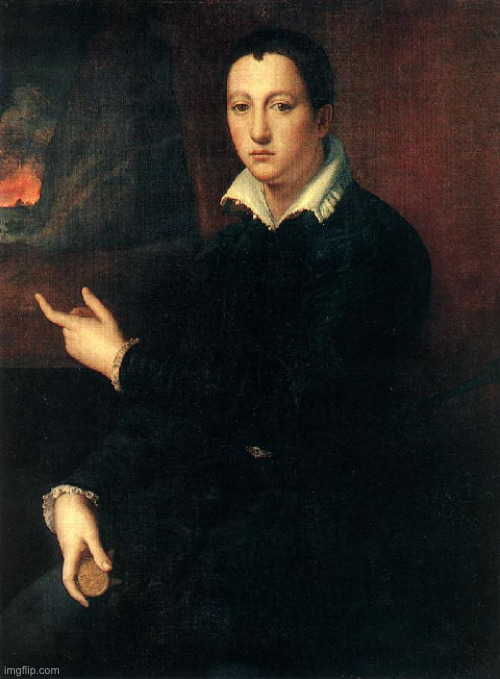
\includegraphics[width=0.25\textwidth]{images/onfireyo.jpg}
\end{center}

\texttt{htop}, Task Manager, etc. will tell you if CPU hosed.


Look at the \%CPU columns and see where all your CPU is going. 



\end{frame}



\begin{frame}[fragile]
\frametitle{Overwatch}



Still, that tells you about right now;  what about the long term average?

Checking with my machine ``Loki'', that has since ascended to Valhalla:\\[1em]

{\scriptsize
\begin{verbatim}
top - 07:28:19 up 151 days, 23:38,  8 users,  load average: 0.87, 0.92, 0.91
\end{verbatim}
}

Those last three numbers are the 1, 5, and 15 minute averages of CPU load.

Lower numbers mean less CPU usage and a less busy machine. 


\end{frame}




\begin{frame}
\frametitle{Interpreting Load Numbers}



Picture a single core of a CPU as a lane of traffic. 

You are a bridge operator and so you need to monitor how many cars are waiting to cross that bridge. 

If no cars are waiting, traffic is good and drivers are happy. 

If there is a backup of cars, then there will be delays.


\end{frame}



\begin{frame}
\frametitle{Single-CPU Load Scheme}



\begin{enumerate}
	\item 0.00 means no traffic. \\
    Anything between 0.00 and 0.99 means we're under capacity and there will be no delay.\\[1em]
	\item 1.00 means we are exactly at capacity. \\
    Everything is okay, but if one more car shows up, there will be a delay.\\[1em]
	\item Anything above 1.00 means there's a backup (delay). \\
    If we have 2.00 load, then the bridge is full and there's an equal number of cars waiting to get on the bridge. 
\end{enumerate}


\end{frame}



\begin{frame}
\frametitle{Car Analogy}

\begin{center}
	\includegraphics[width=\textwidth]{images/car-analogy.png}
\end{center}

\end{frame}



\begin{frame}
\frametitle{Is it a Problem?}



$\ge$ 1.00 isn't necessarily bad, but you should be concerned if there is consistent load of 1.00 or above. 

$<$ 1.00 but getting close to it: you know how much room you have to scale things up.

$>$ 0.70 then it's probably time to investigate.

$\ge$ 1.00 consistently we have a serious problem. 

5.00: this is a red alert situation.


\end{frame}



\begin{frame}
\frametitle{Multicore}



Now this is for a single CPU---if you have a load of 3.00 and a quad core CPU, this is okay. 

Traffic analogy: four lanes of traffic, of which 3 are being used to capacity.

So we have a 4th lane free and it's as if we're at 75\% utilization on a single CPU.


\end{frame}

\begin{frame}
\frametitle{Memory?}

Using garbage collection? Is it running a lot?

\begin{center}
  
\includegraphics[width=0.5\textwidth]{images/undertaker.jpg}
\end{center}

Out of memory errors (crash or recovery)?

\end{frame}


\begin{frame}[fragile]
\frametitle{Disk? Or Memory?}



How to tell? Look at disk utilization. \\[1em]

Not enough RAM $\Rightarrow$ swapping, bad perf, no scalability.\\[1em]

(In the worst case.)\\[1em]

You can ask via \texttt{top} about how much swap is being used, but that's probably not the interesting value. 

{\scriptsize
\begin{verbatim}
KiB Mem:   8167736 total,  6754408 used,  1413328 free,   172256 buffers
KiB Swap:  8378364 total,  1313972 used,  7064392 free.  2084336 cached Mem
\end{verbatim}
}


\end{frame}



\begin{frame}
\frametitle{Misleading Memory}



Why? Memory being ``full'' does not necessarily mean anything bad. \\[1em]

It means the resource is being used to its maximum potential, yes, but there is no benefit to keeping a block of memory open for no reason. (Or stockpiling late days).\\[1em]

Also, memory is unlike CPU; if there's nothing for the CPU to do, it will just idle (low power state).


\end{frame}


\begin{frame}
\frametitle{Really, Dvorak, Really?}



Memory won't ``forget'' data if it doesn't happen to be needed right now---data will hang around in memory until there is a reason to move or change it. 

So freaking out about memory appearing as full is kind of like getting all in a knot about how ``System Idle Process'' is hammering the CPU\ldots


\end{frame}




\begin{frame}
\frametitle{Page Faults}



You can also ask about page faults, with the command
\begin{center}
\texttt{ps -eo min\_flt,maj\_flt,cmd}
\end{center}

Major page faults: had to fetch from disk. 

Minor page faults: had to copy a page from another process. 

The output of this is too big even for the notes.

This is process-lifetime data.

\end{frame}



\begin{frame}[fragile]
\frametitle{Swapping Report}



What you really want is to ask Linux for a report on swapping:

\vspace*{-2em}
{\scriptsize
\begin{verbatim}
jz@Loki:~$ vmstat 5
procs -----------memory---------- ---swap-- -----io---- -system-- ------cpu-----
 r  b   swpd   free   buff  cache   si   so    bi    bo   in   cs us sy id wa st
 1  0 1313972 1414600 172232 2084296    0    0     3    39    1    1 27  1 72  0  0
 0  0 1313972 1414476 172232 2084296    0    0     0    21  359  735 19  0 80  0  0
 0  0 1313972 1414656 172236 2084228    0    0     0   102  388  758 22  0 78  0  0
 4  0 1313972 1414592 172240 2084292    0    0     0    16  501  847 33  0 67  0  0
 0  0 1313972 1412028 172240 2084296    0    0     0     0  459  814 29  0 71  0  0
\end{verbatim}
}

\end{frame}



\begin{frame}[fragile]
\frametitle{Swapping Report with Actual Swapping}

{\small
\begin{verbatim}
  procs                      memory    swap          io     system cpu
r  b  w   swpd   free  buff cache  si  so   bi   bo   in    cs us  sy  id
. . .
1  0  0  13344   1444  1308 19692   0 168  129   42 1505   713 20  11  69
1  0  0  13856   1640  1308 18524  64 516  379  129 4341   646 24  34  42
3  0  0  13856   1084  1308 18316  56  64   14    0  320  1022 84   9   8
\end{verbatim}
}

\end{frame}



\begin{frame}
\frametitle{Skip to Disk}



Looking at disk might seem slightly redundant if memory is not the limiting factor. 

After all, if the data were in memory it would be unnecessary to go to disk in the first place. 

Still, sometimes we can take a look at the disk and see if that is our bottleneck.


\end{frame}




\begin{frame}[fragile]
\frametitle{Looking at Disk Usage}

{\tiny
\begin{verbatim}
jz@Loki:~$ iostat -dx /dev/sda 5 
Linux 3.13.0-24-generic (Loki) 	16-02-13 	_x86_64_	(4 CPU)

Device:         rrqm/s   wrqm/s     r/s     w/s    rkB/s    wkB/s avgrq-sz avgqu-sz   await r_await w_await  svctm  %util
sda               0.24     2.78    0.45    2.40    11.60   154.98   116.91     0.17   61.07   11.57   70.27   4.70   1.34
\end{verbatim}
}



Last column \%util tells us what we want to know.


\end{frame}



\begin{frame}[fragile]
\frametitle{Network}



We can ask about the network with \texttt{nload}. 
 
You get a nice little graph if there is anything to see. 

But you'll get the summary, at least:

\begin{verbatim}
Curr: 3.32 kBit/s
Avg: 2.95 kBit/s
Min: 1.02 kBit/s
Max: 12.60 kBit/s
Ttl: 39.76 GByte                                                                                       \end{verbatim}

\end{frame}

\begin{frame}
\frametitle{Physical Limitations}

If we saw data leaving at 100 MBit, might be clear it's the max.

But what if you're using other hardware?
\begin{center}
  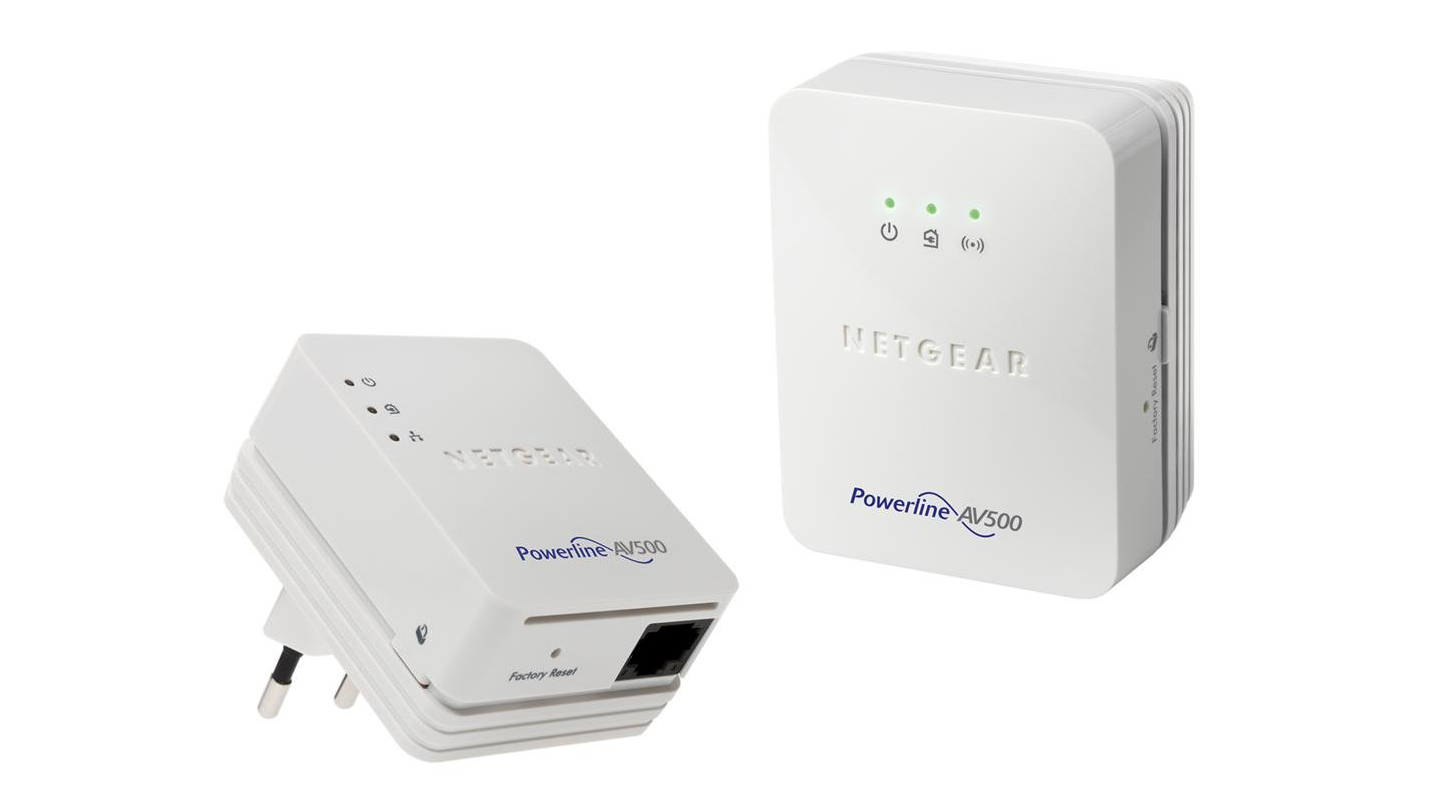
\includegraphics[width=0.4\textwidth]{images/powerline.jpg}
\end{center}

Same for wireless networks... walls, floors, EM interference...

\end{frame}

\begin{frame}
\frametitle{Testing Speed}

How to test? Use tools like speedtest.net

\begin{center}
  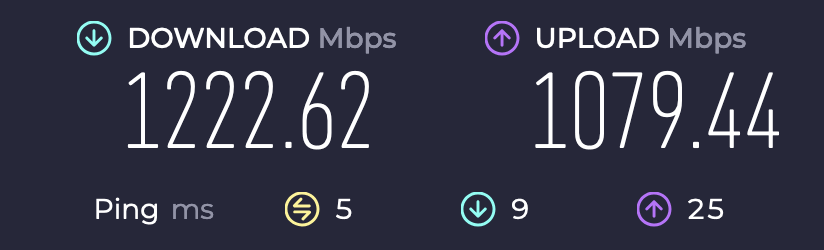
\includegraphics[width=0.5\textwidth]{images/speedtest.png}
\end{center}

Need to test multiple times.

Good results doesn't necessarily mean good performance.

\end{frame}

\begin{frame}[fragile]
\frametitle{Traceroute}

If you want to get an idea of the path and the latency to a particular remote system, you can use the \texttt{traceroute} tool.

{\scriptsize
\begin{verbatim}
Microsoft Windows [Version 10.0.19043.1288]
(c) Microsoft Corporation. All rights reserved.
C:\Users\Michael>tracert catchpoint.com
Tracing route to catchpoint.com [64.79.149.76]
Over a maximum of 30 hops: 
1	2ms	1ms	1ms 10.0.0.1
2 	10ms	10ms	10ms 96.120.40.245
3	10ms	11ms	12ms	96.110.175.85
4	10ms	16ms	10ms 	162.151.63.57
5	19ms	16ms	20ms	96.108.21.57
6	15ms	19ms	14ms	96.216.134.10
7          	19ms 	22ms 	21ms 	be-32121-cs02.350ecermak.il.ibone.comcast.net [96.110.42.181]
8          	22ms 	34ms 	22ms 	be-2204-pe04.350ecermak.il.ibone.comcast.net [96.110.37.38]
9          	22ms 	20ms 	20ms 	50.208.234.106
10       	51ms 	50ms 	49ms 	ae18-0.cr02.dlls02-tx.us.windstream.net [40.128.10.135]
11       	73ms 	72ms 	72ms 	ae4-0.agr03.phnd01-az.us.windstream.net [169.130.193.231]
12       	84ms 	73ms 	75ms 	ae1-0.pe05.phnd01-az.us.windstream.net [169.130.169.31]
13       	85ms 	84ms 	85ms 	h241.23.132.40.static.ip.windstream.net [40.132.23.241]
14       	*         	82ms 	78ms 	be181.las-n10s1-core1.switch.com [66.209.64.121]
15       	79ms 	77ms 	80ms 	bell011.las-agg7s5-1.switch.com [66.209.72.26]
16       	79ms 	77ms 	79ms 	64.79.139.18
17       	77ms 	77ms 	87ms 	64.19.149.76
Trace complete
\end{verbatim}
}

\end{frame}

\begin{frame}
\frametitle{Latency \& Loss}

Latency can never get down to 0: speed of light limitation.

Example: New York to Lyon is 73.21ms which is something like 83.79\% of the speed of light in fibre-optic cable (as of August 2024).

Another cause: packet loss! Requires re-sending data...\\
\quad Replace dying devices? Environmental causes?

\end{frame}


\begin{frame}
\frametitle{Locks}

Maybe our code is slow because we are waiting for locks?

\begin{center}
	\includegraphics[width=0.5\textwidth]{images/letmein.png}
\end{center}

Out of scope: deadlock detection.

\end{frame}


\begin{frame}
\frametitle{How to Find It?}

Unexpectedly low CPU usage not explained by I/O-waiting?

Many threads blocked?

No magical \texttt{locktrace} tool -- may need our own tracing.

\texttt{perf lock} is for kernel locks; VTune costs money.

\end{frame}


\begin{frame}
\frametitle{Probably it's CPU}

Most of our discussion will be about CPU though.

\begin{center}
  
\includegraphics[width=0.5\textwidth]{images/sabotage.jpg}
\end{center}

Why? That's probably what it is!


\end{frame}

\end{document}